\section{Rešitev}
Najprej si poglejmo hitrost različnih funkciji. Funkciji \verb|QR| in \verb|QR_trid|
so napisane s pomočjo primera na spletni učilnici. Postopek \verb|QR| uporablja
razcep QR in iterativno dobimo lastne vrednosti po diagonali, če spremenimo začetno matriko v $A=RQ$.
Druga metoda, pa je deluje preko tridiagonalizacije in Hausholderjevih zrcaljen. Slednja metoda
deluje le ko je matrika simetrična.

\begin{figure}[h]
    \centering
    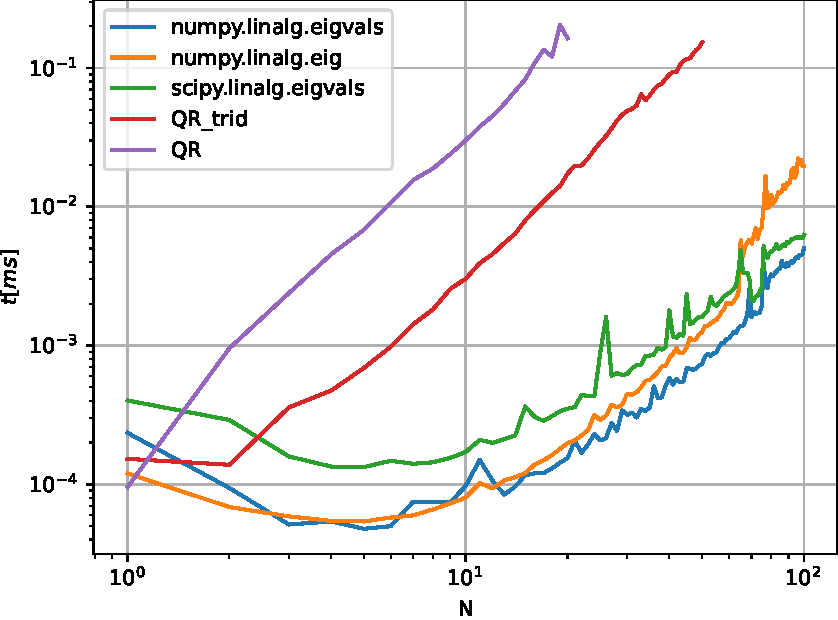
\includegraphics[width=77mm]{pdfs/t(N).pdf}
    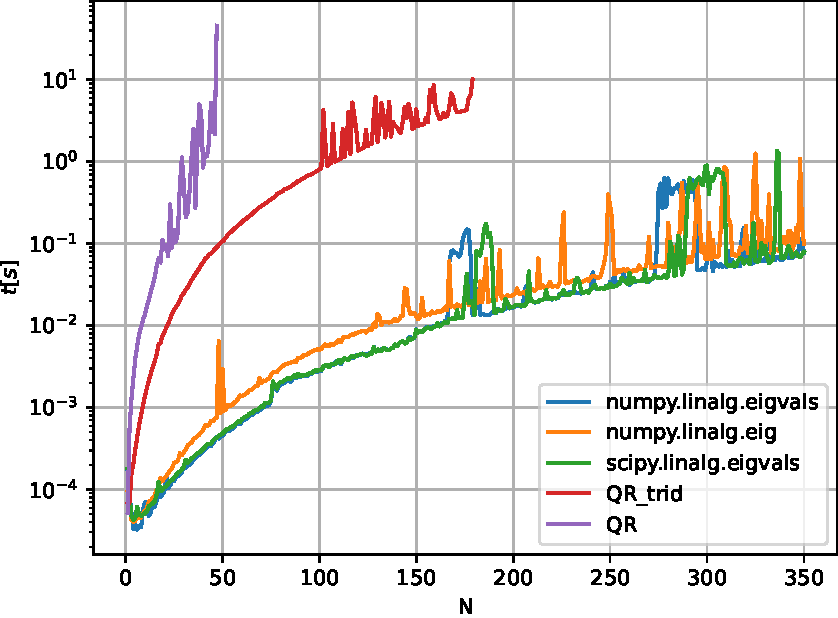
\includegraphics[width=77mm]{pdfs/t(N)log.pdf}
    \caption{Hitrost algoritmov v odvisnosti velikosti matrike}
\end{figure}

Vidimo, da je najhitrejša metoda \verb|scipy.linalg.eigvals()|, zato jo
v nadeljevanju uporabimo.

Poglejmo si še odvisnost najnižjih energijskih spektrov od
parametra $\lambda$ in kako smo definirali matrične elemente
hamiljtonjanke.

\begin{figure}[h]
    \centering
    \subfigure{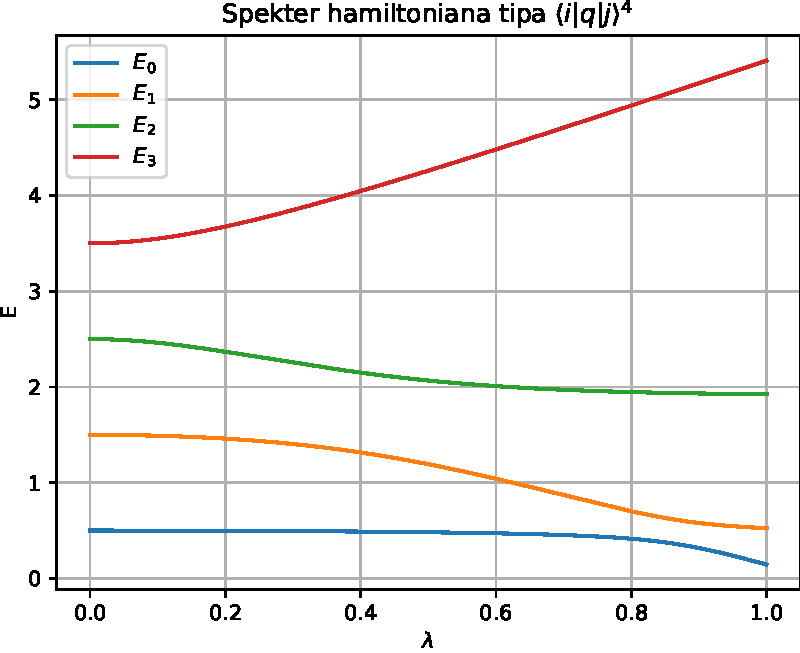
\includegraphics[width=0.32\textwidth]{pdfs/spekter_1.pdf}}
    \subfigure{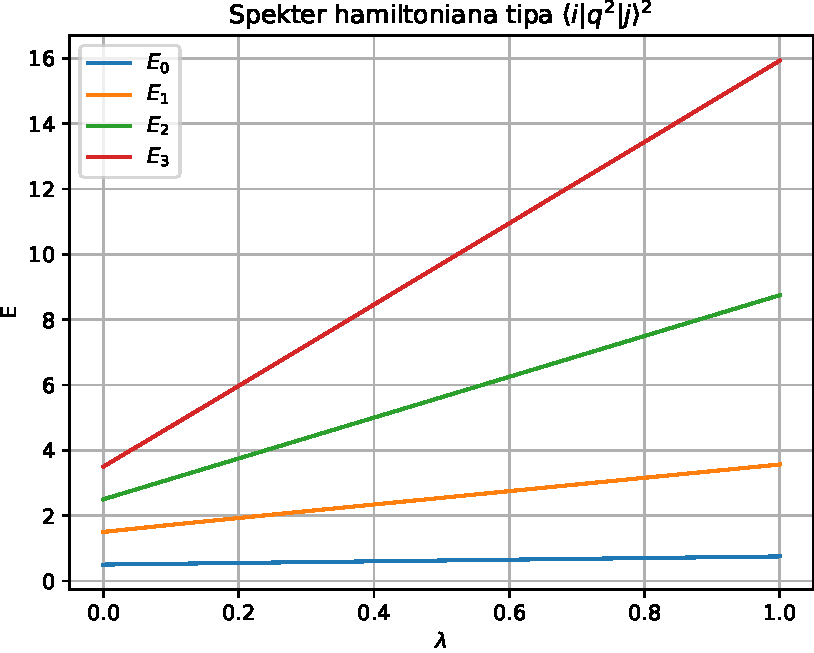
\includegraphics[width=0.32\textwidth]{pdfs/spekter_2.pdf}}
    \subfigure{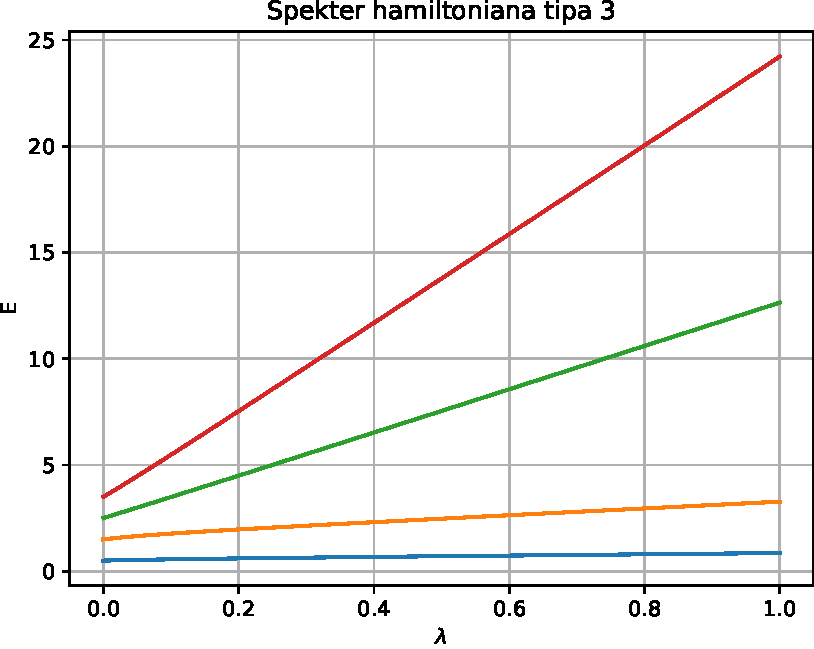
\includegraphics[width=0.32\textwidth]{pdfs/spekter_3.pdf}}
    \caption{Energijski spekter v odvisnosti parametra $\lambda$}
\end{figure}
\newpage
Kako pa lastne energije konvergirajo s povečavo hamiltonjana?
\begin{figure}[h]
    \begin{center}
        \subfigure{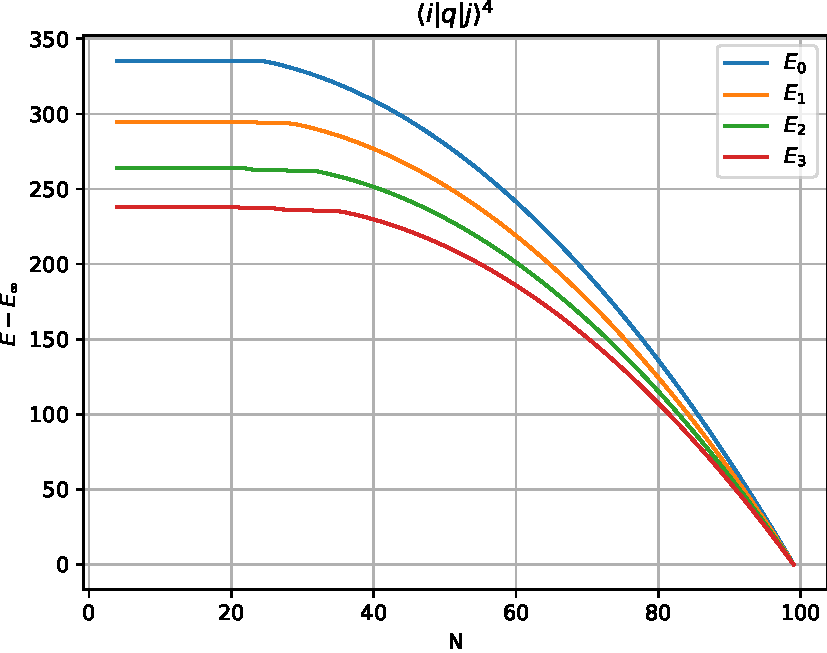
\includegraphics[width=0.32\textwidth]{pdfs/E(N)0.pdf}}
        \subfigure{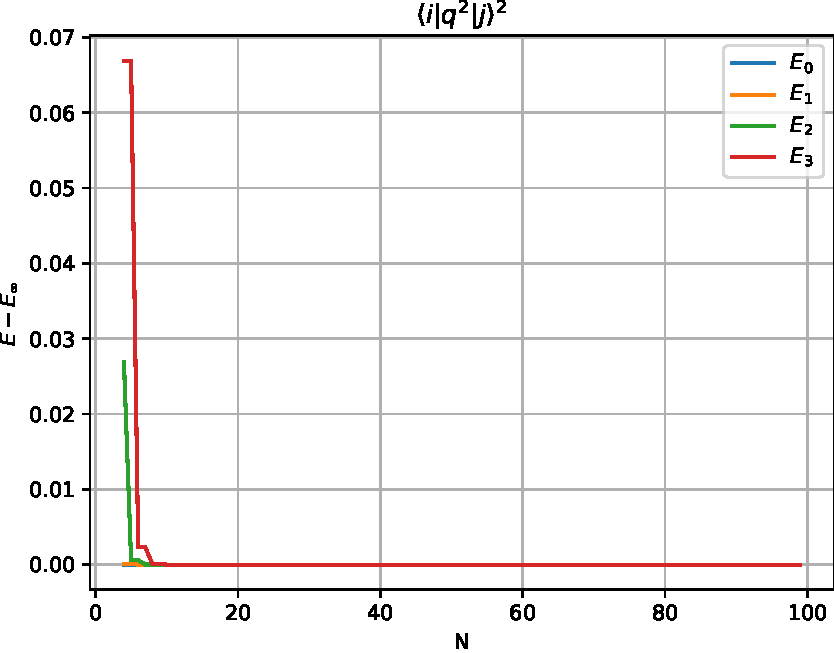
\includegraphics[width=0.32\textwidth]{pdfs/E(N)1.pdf}}
        \subfigure{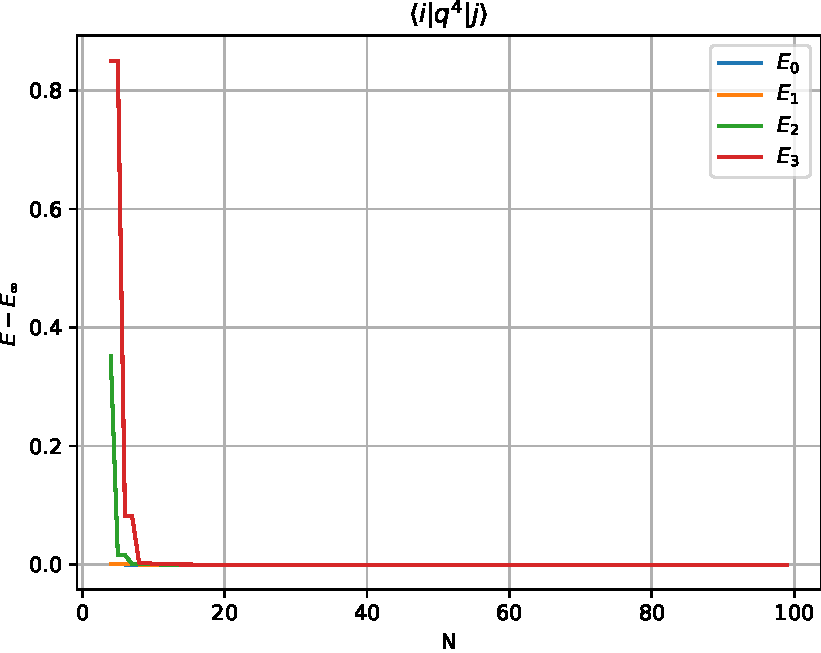
\includegraphics[width=0.32\textwidth]{pdfs/E(N)2.pdf}}
    \end{center}
    \caption{Spreminjanje energijskega spektra prvih štirih energij v odvisnosti velikosti hamiltonjana}
\end{figure}
Ker dva grafa nista najbolj pregledna si poglejmo še logaritemsko skalo.
\begin{figure}[h]
    \begin{center}
        \subfigure{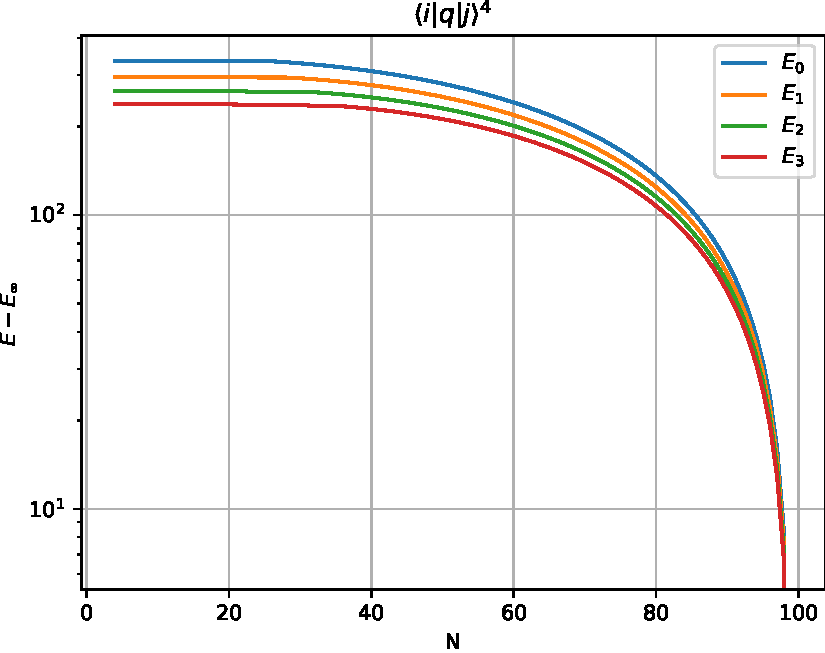
\includegraphics[width=0.32\textwidth]{pdfs/log(E(N))0.pdf}}
        \subfigure{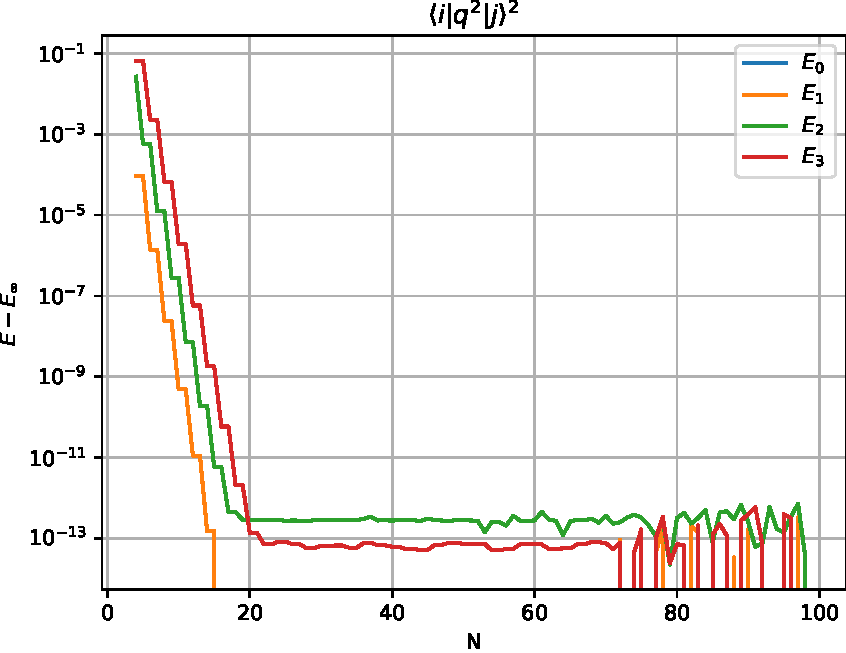
\includegraphics[width=0.32\textwidth]{pdfs/log(E(N))1.pdf}}
        \subfigure{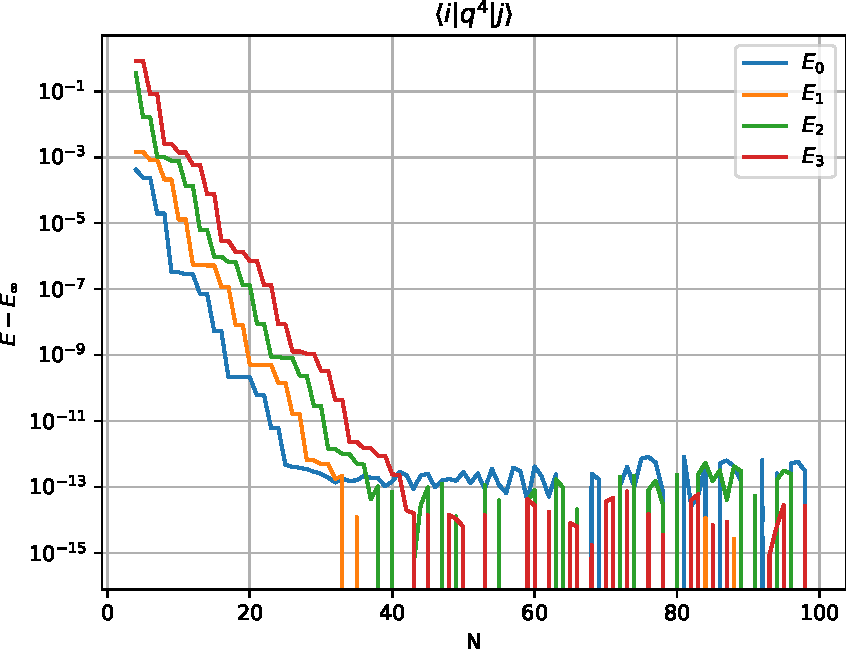
\includegraphics[width=0.32\textwidth]{pdfs/log(E(N))2.pdf}}
    \end{center}
    \caption{Spreminjanje energijskega spektra prvih štirih energij v odvisnosti velikosti hamiltonjana v logaritemski skali}
\end{figure}
Vidimo, da najhitreje konvergira matrika z elementi $H_{ij} = \langle i | q^2 | j \rangle^2 $.